\documentclass[graphics]{beamer}

\usepackage{graphicx}
\usepackage{verbatim}
\usepackage{wrapfig}
\useoutertheme{shadow}
%\usecolortheme{orchid}
\usecolortheme{seahorse}


% math commands
\newcommand{\be}{\begin{eqnarray}}
\newcommand{\ee}{\end{eqnarray}}
\newcommand{\beq}{\begin{equation}}
\newcommand{\eeq}{\end{equation}}
\def\simless{\mathbin{\lower 3pt\hbox
      {$\rlap{\raise 5pt\hbox{$\char'074$}}\mathchar"7218$}}}
\def\simgreat{\mathbin{\lower 3pt\hbox
      {$\rlap{\raise 5pt\hbox{$\char'076$}}\mathchar"7218$}}} %> or of order

% variables

\def\toonscale{0.45}
\def\mboxy#1{\mbox{\small #1}}


\begin{comment}
\AtBeginSection[]{
  \frame{
    \frametitle{Outline}
    \tableofcontents[currentsection]
  }
}
\end{comment}

\title{Galaxy Torques
}
\subtitle{}
\author[U. Pen]{\textcolor{green}{Ue-Li Pen, Haoran Yu, Pavel Motloch}
\\[8mm] 
}
\date{June 4, 2019}


\begin{document}

\frame{
\begin{picture}(320,250)
\put(-50,-130){
\includegraphics[width=5.5in]{Figures/delta_nu_sim.pdf}}
\end{picture}
\vspace{-3in}
\titlepage
}

%\section*{Introduction}
\section{Galaxy angular momentum}

\begin{comment}
  \subsection{Outline}

  \frame{
    \frametitle{Outline}
    \tableofcontents
  }
\end{comment}

\frame{
    \frametitle{Prograde Winding}
\includegraphics[width=4.1in]{Figures/M51s.jpg}  

(from Wikipedia)
  }

\frame{
    \frametitle{Prograde Winding}
\includegraphics[width=4.1in]{Figures/M51s.jpg}  

(M51, from Wikipedia)
  }

\frame{
    \frametitle{Tilt}
\includegraphics[width=4.1in]{Figures/AndromedaGalaxy.jpg}  

(from Wikipedia)
  }
\frame{
    \frametitle{Tilt}
\includegraphics[width=4.1in]{Figures/AndromedaGalaxy.jpg}  

(M31, from Wikipedia)
  }

  \frame{
    \frametitle{Galaxy Spins}
    \begin{itemize}
        \item most galaxies are rotating disks of stars and gas
        \item readily identifyable spin axis
        \item dust lanes, trailing spiral arms, (HI) velocity (rotation) field
     \end{itemize}
}

  \frame{
    \frametitle{Observables}
    \begin{itemize}
        \item ellipticity
        \item position angle
        \item winding direction (S vs Z)
        \item reddening
        \item human and machine classifications for $10^{4-6}$ objects
          (galaxy zoo, Land+ 2008 )
    \end{itemize}
}
\frame{
    \frametitle{Zoo}
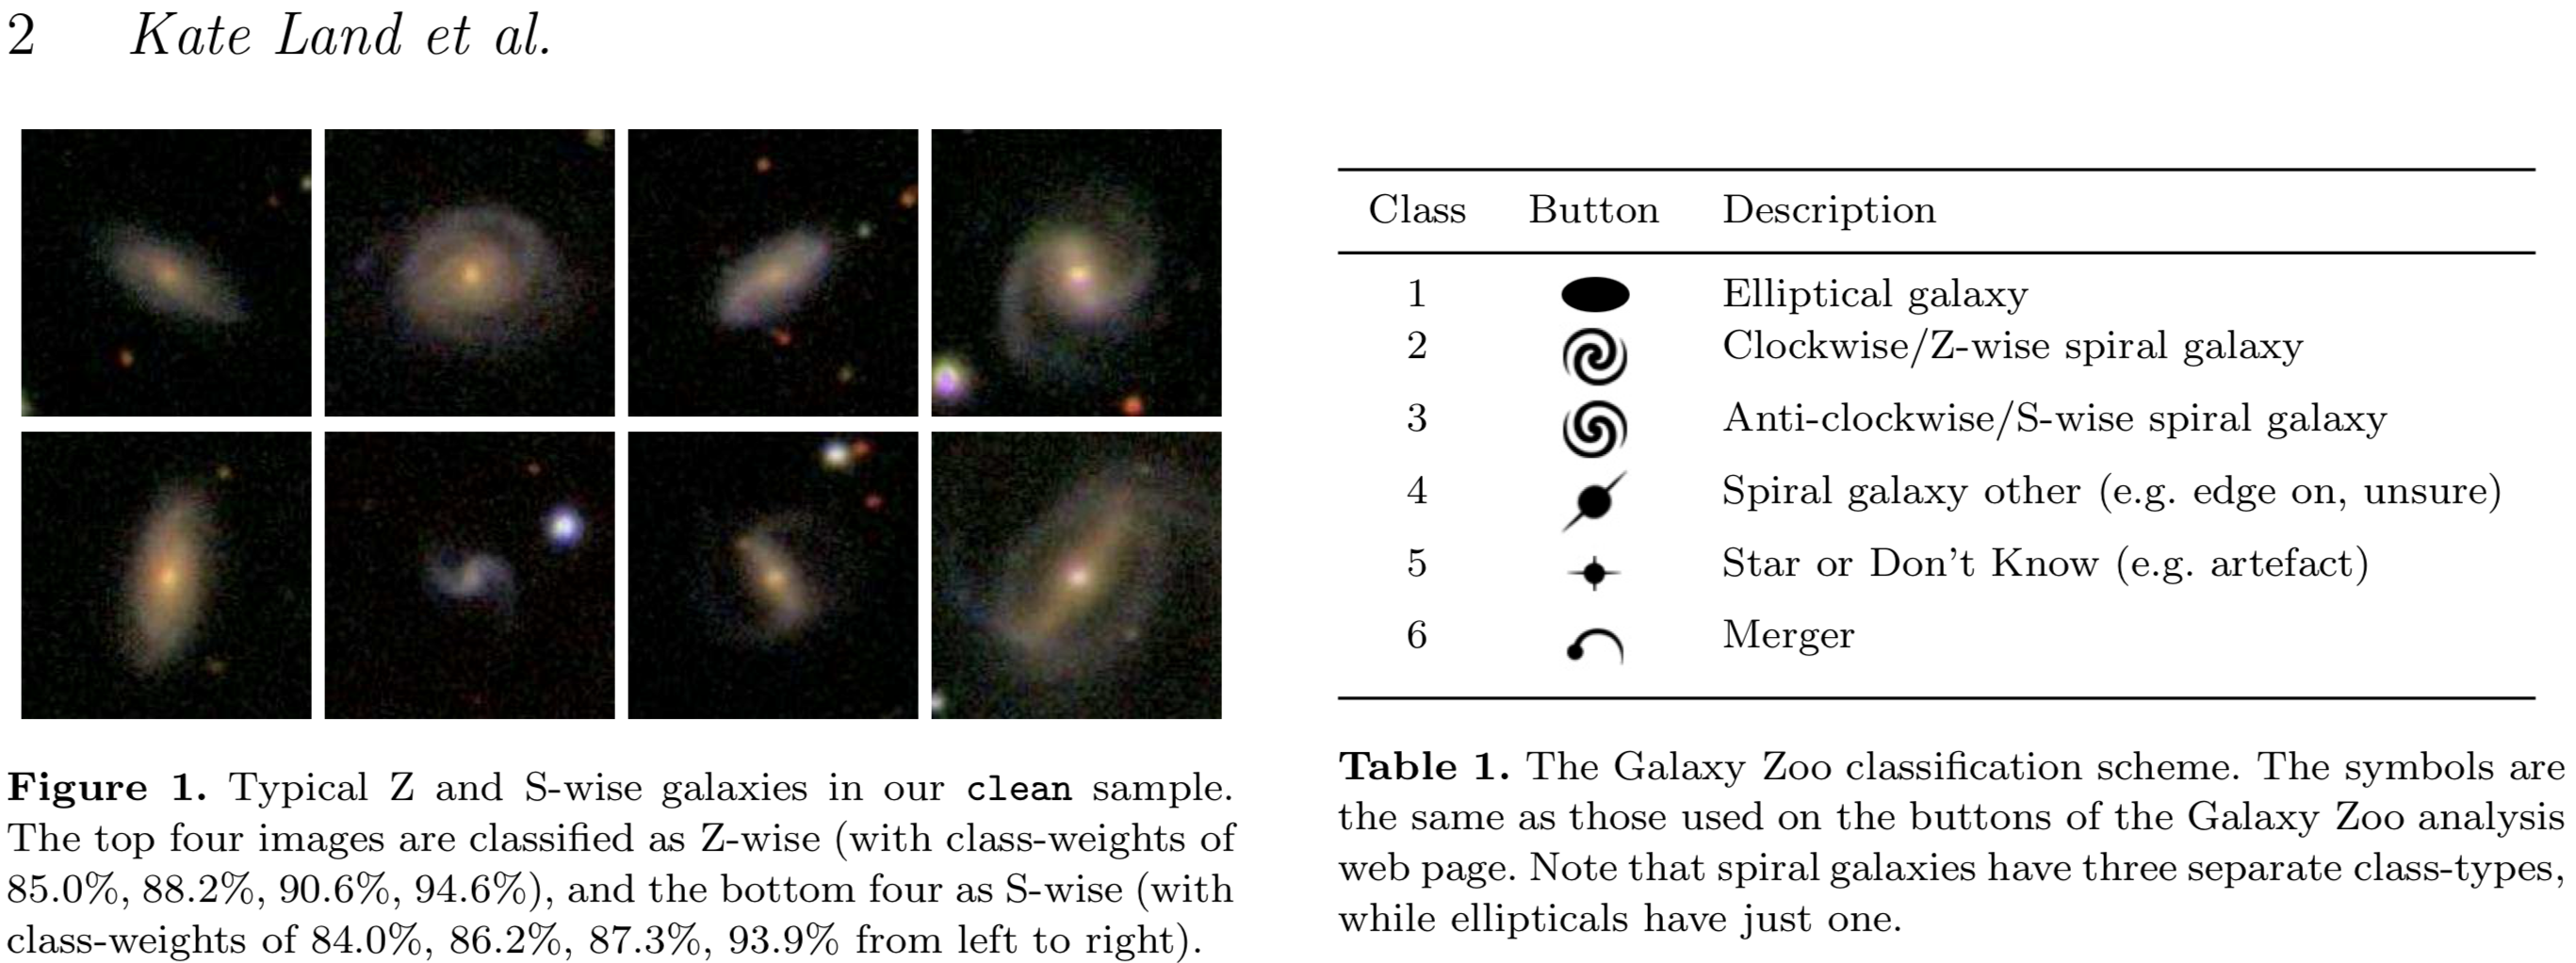
\includegraphics[width=4.1in]{Figures/land2008.png}  
  }
\frame{
    \frametitle{GAMA}
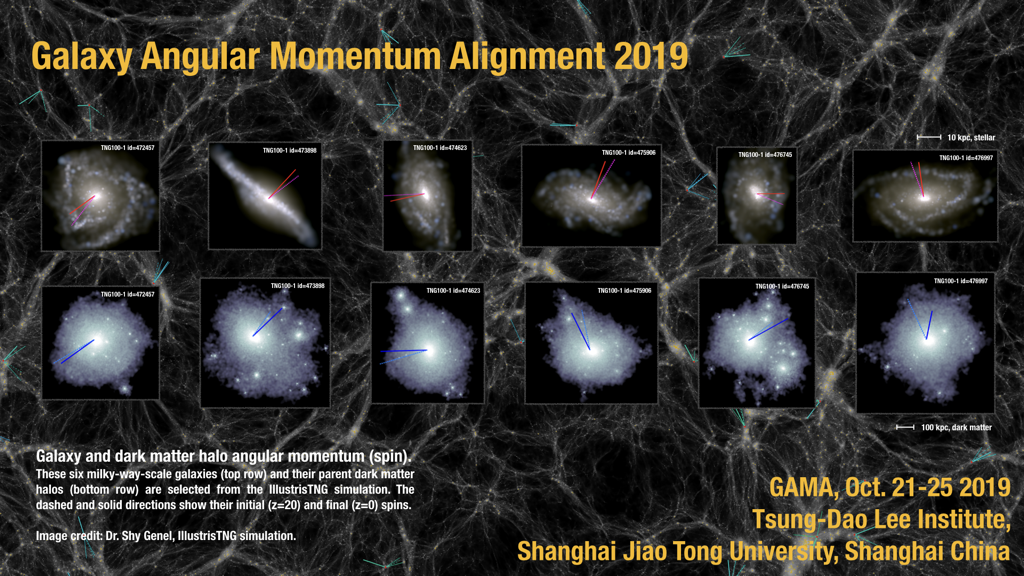
\includegraphics[width=4.1in]{Figures/GAMA.png}  
  }

  \frame{
    \frametitle{Context}
    \begin{itemize}
        \item S White 1984: TTT
        \item Genel++: spin magnitude
        \item Lee\&Pen 2000: LSS statistical theory
        \item Yu++ 2018: Lagrangian theory, high fidelity direction
          memory, poor magnitude memory
     \end{itemize}
}


  \frame{
    \frametitle{Angular momentum}
    \begin{itemize}
        \item 1st order effect from misalignment of moment of inertia
          and tidal tensor
        \item torque: $\tau\equiv\int \rho \bf{r} \times \nabla \phi$
        \item Taylor expand: $\tau_i=\epsilon_{ijk} \int \rho x^jx^l \partial_l\partial_k\phi \equiv\epsilon_{ijk} I_{il}T_{lk}$
        \item Tensor form $\tau= * I \cdot T$
        \item first realized by S. White (1984), see also LP00
     \end{itemize}
}

\frame{
    \frametitle{3-D: E-mode}
%\vspace{-0.5in}
\hspace{-0.2in}\includegraphics[width=2.3in]{Figures/nonlinear.png}  
\vspace{0.15in}\includegraphics[width=2.21in]{Figures/reconstructed.png}  

Eulerian (L) vs Lagrangian (R) (from Yu et al 2016, 1610.7112)
  }

  \frame{
    \frametitle{Tensors}
    \begin{itemize}
        \item Tide: ${\bf T}$ reconstructed from density field
        \item Inertia: non-linear reconstruction of ${\bf I}$
        \item strongly correlated
     \end{itemize}
}
\frame{
    \frametitle{Sim}
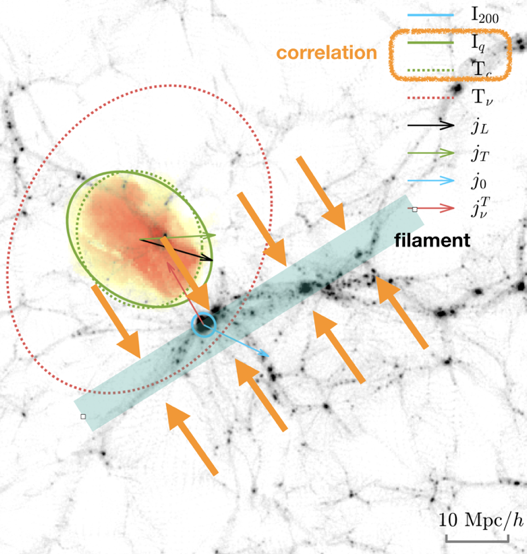
\includegraphics[width=4.1in]{Figures/I-T.png}  
Yu+2018
  }

\frame{
    \frametitle{Lagrangian coordinates}
\center{\includegraphics[width=4.3in]{Figures/delta_reco_raw.pdf}  }
  }

  \frame{
    \frametitle{Coordinate freedom}
\begin{eqnarray}
{\rm potential\ deformation\ \ \ \ \ }  x^i &=& \xi^\mu \delta^i_\mu + \frac{\partial \phi}{\partial
    \xi^\mu}\delta^{i\mu}\nonumber\\
{\rm dreibein\ \ \ \ \ \  } e^i_\mu &\equiv& \partial x^i / \partial \xi ^ \mu \nonumber\\
 {\rm volume\  element\ \ \ \ }\sqrt{g} &\equiv& \mathrm{det}\left| e^i_\mu\right|\nonumber\\
{\rm mass\ coordinate \ \ \ \ \ }    \rho \sqrt{g}&=&\mathrm{Const.}\nonumber\\
    \partial _\mu (\rho \sqrt{g} e^\mu _i \delta^{i\nu}
    \partial_\nu \dot{\phi})&=&\langle\rho\rangle-\rho \sqrt{g}
\label{eqn:dif}
\end{eqnarray}
Solve Monge-Amp\'ere eqn (\ref{eqn:dif}) using multigrid (Pen 1995):
unique bijective mass coordinate.  See also Tully/Peebles, Mohayaee+, Goldberg, Schmidtfull, Wang+, Seljak,
Zaldarriaga, Hada/Eisenstein, Shi/Brikin/Li+, Jasche+, Sarpa+
}

  \frame{
    \frametitle{Multigrid solution}
\vspace{-0.7in}\center{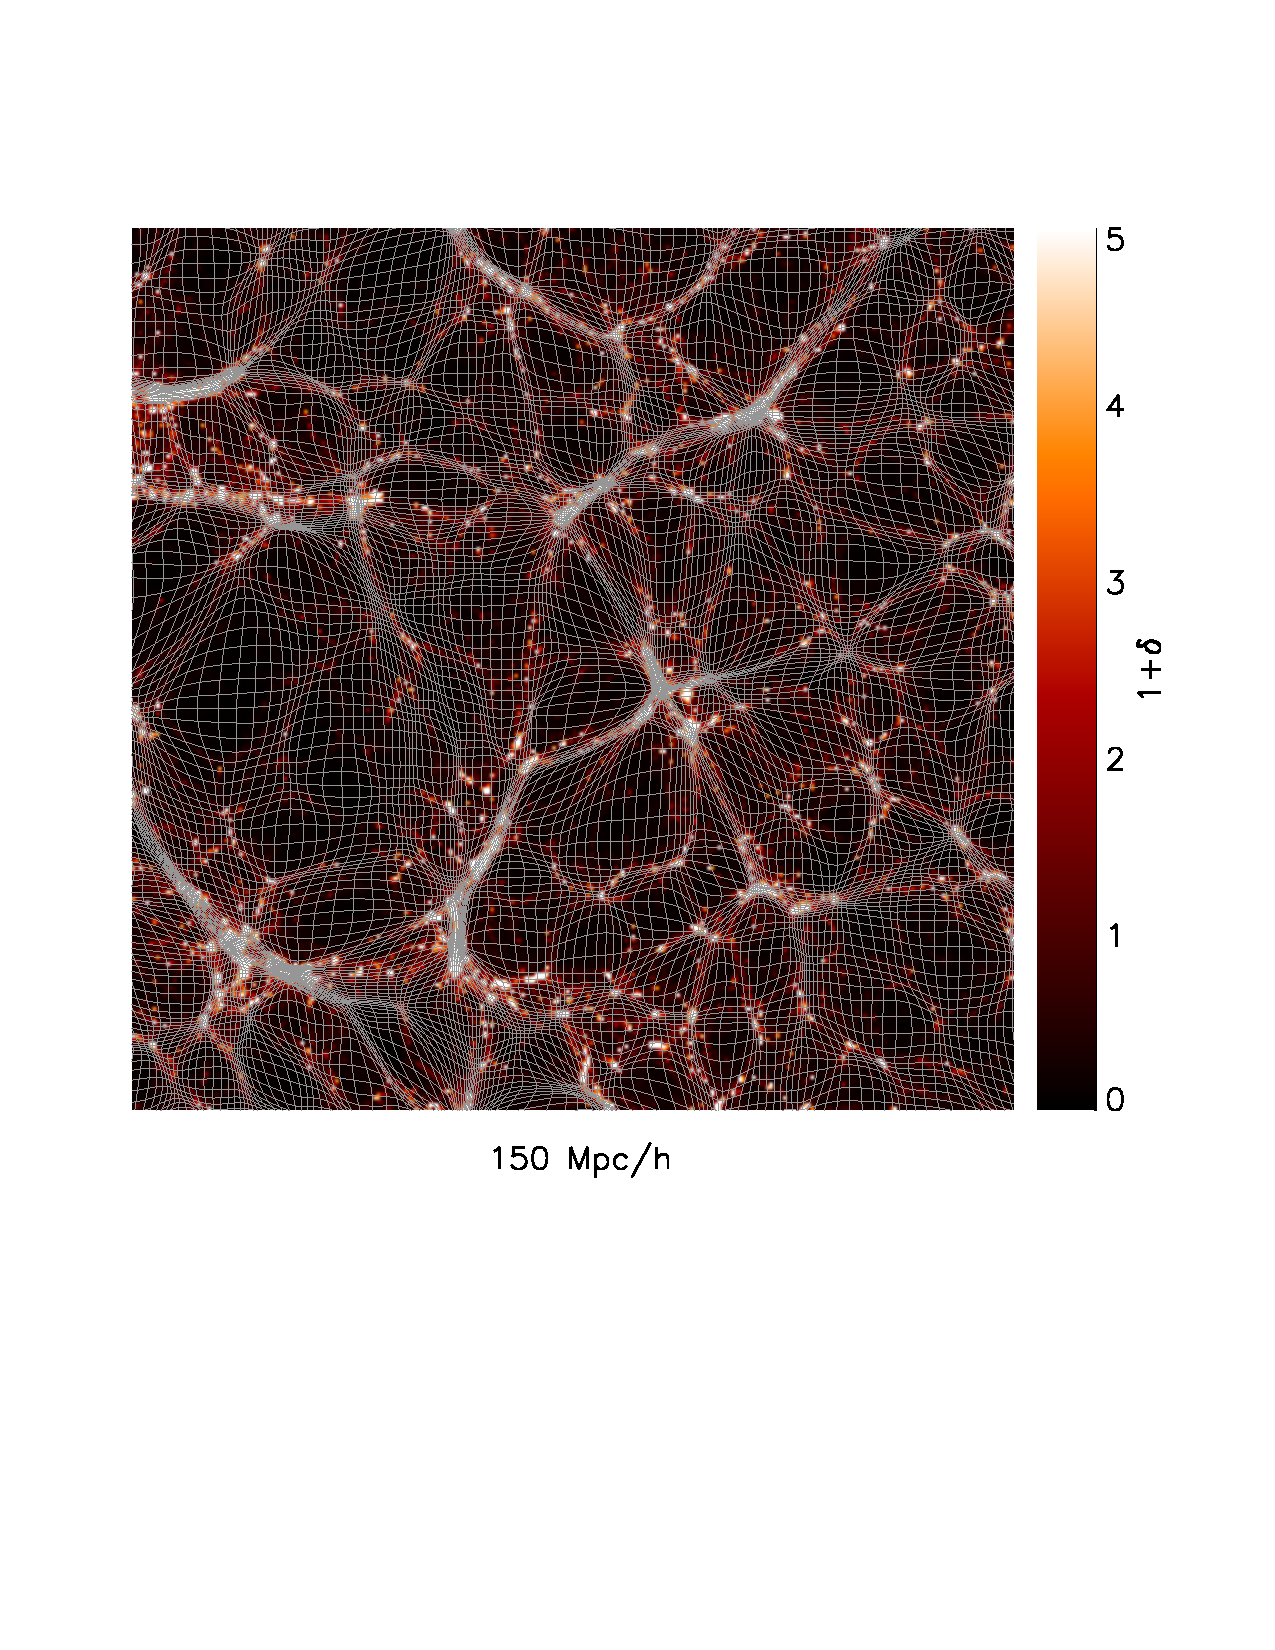
\includegraphics[width=4.0in]{Figures/map0512-0128_i1500_xz222.pdf}}
Zhu et al 1610.09638
}
  \frame{
    \frametitle{Redshift space}
Zhu et al 1610.09638
\vspace{-0.7in}\center{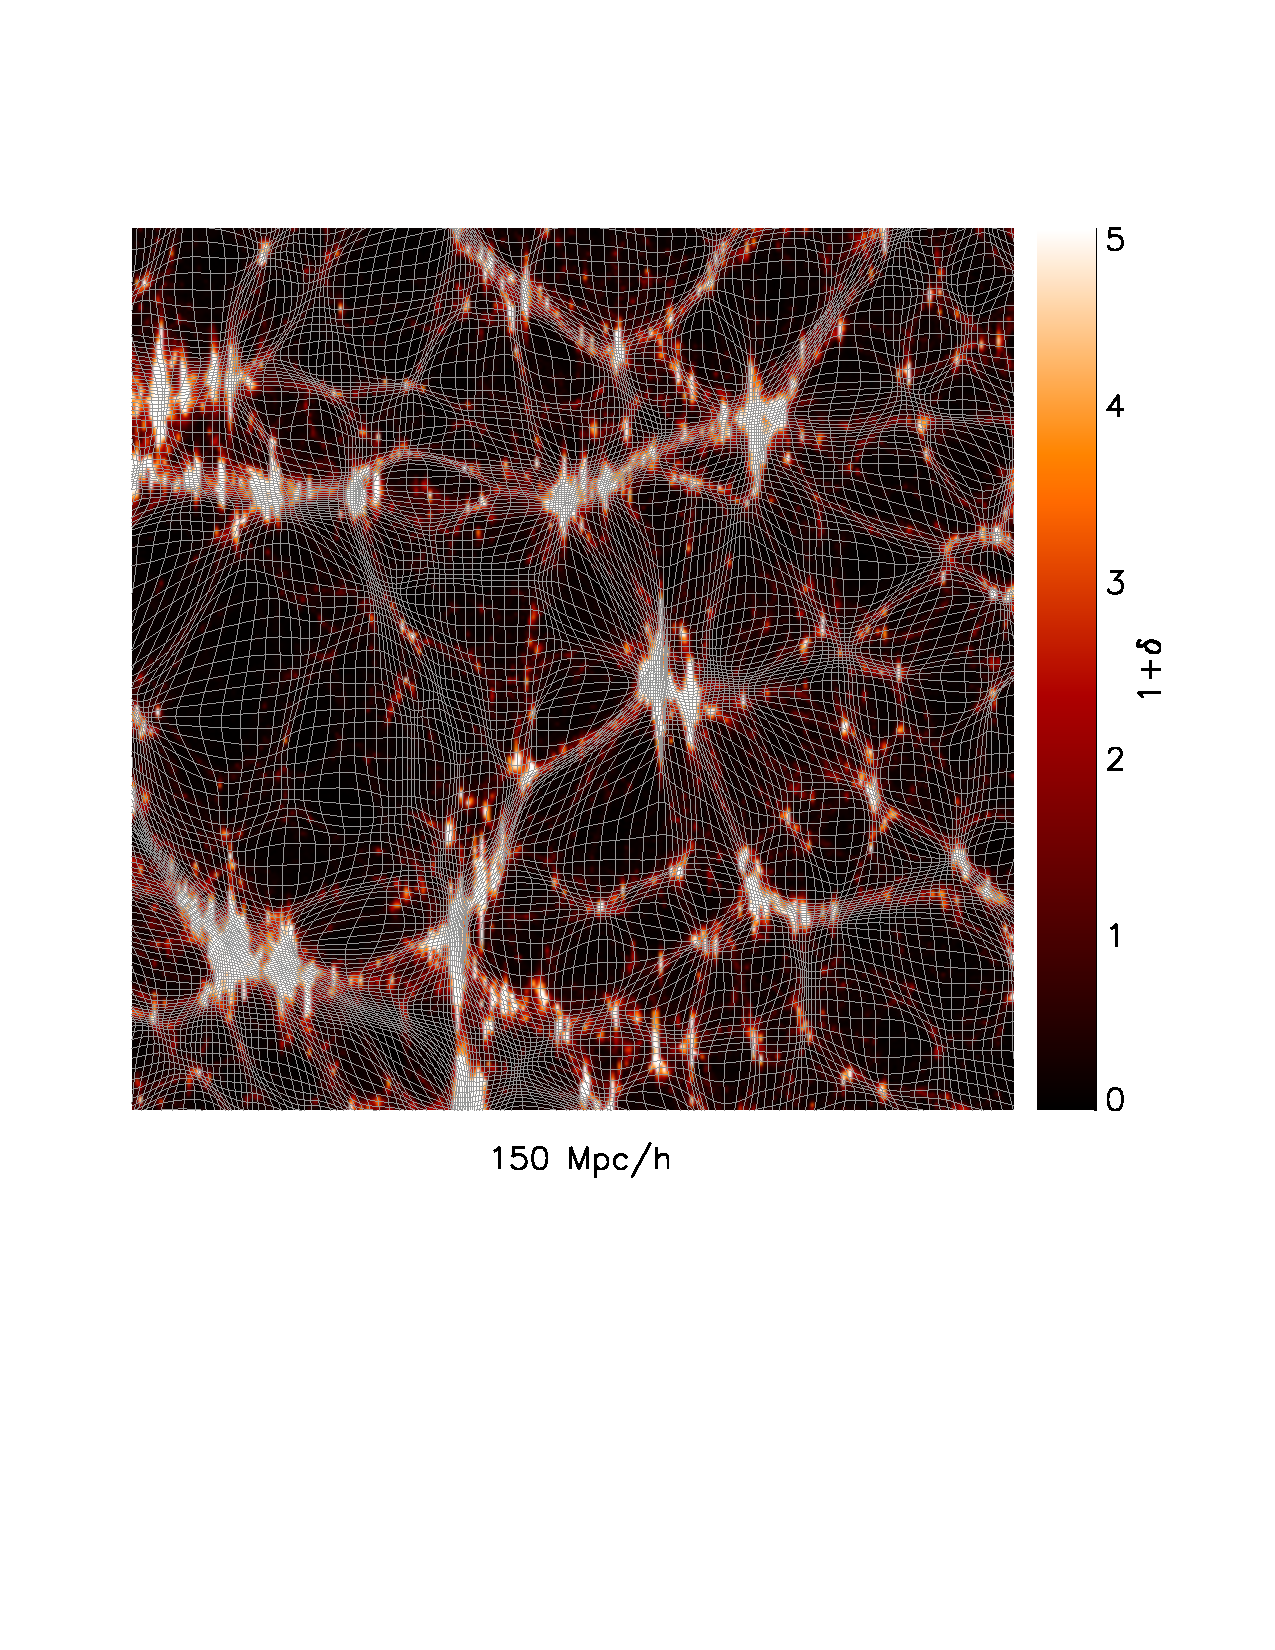
\includegraphics[width=4.0in]{Figures/map0512-0128_i0900_xz222_rsd3.pdf}}
}

  \frame{
    \frametitle{Low noise limit}
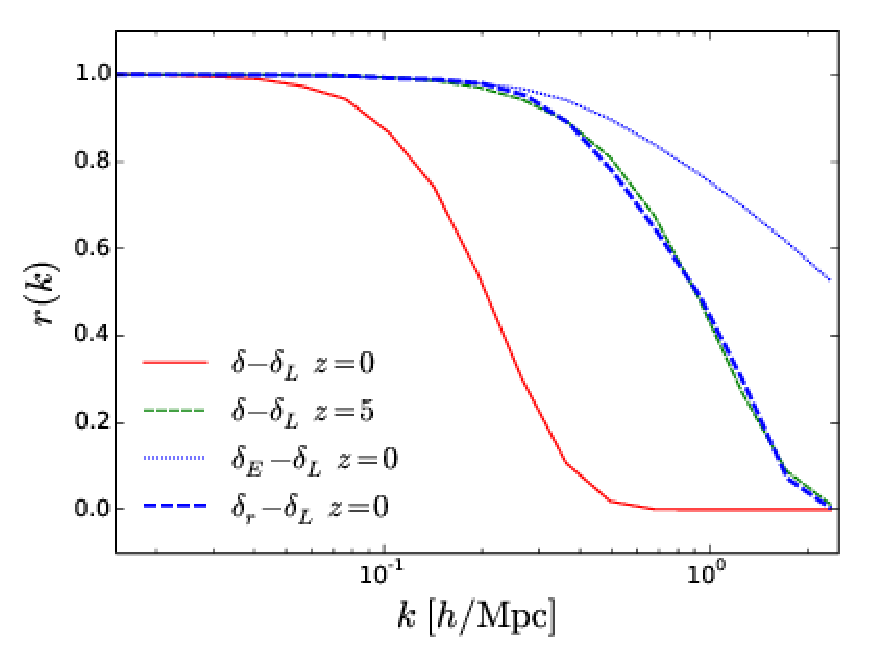
\includegraphics[width=3.4in]{Figures/rk.pdf}
}
  \frame{
    \frametitle{Halos}
\vspace{-0.5in}\hspace{-0.9in}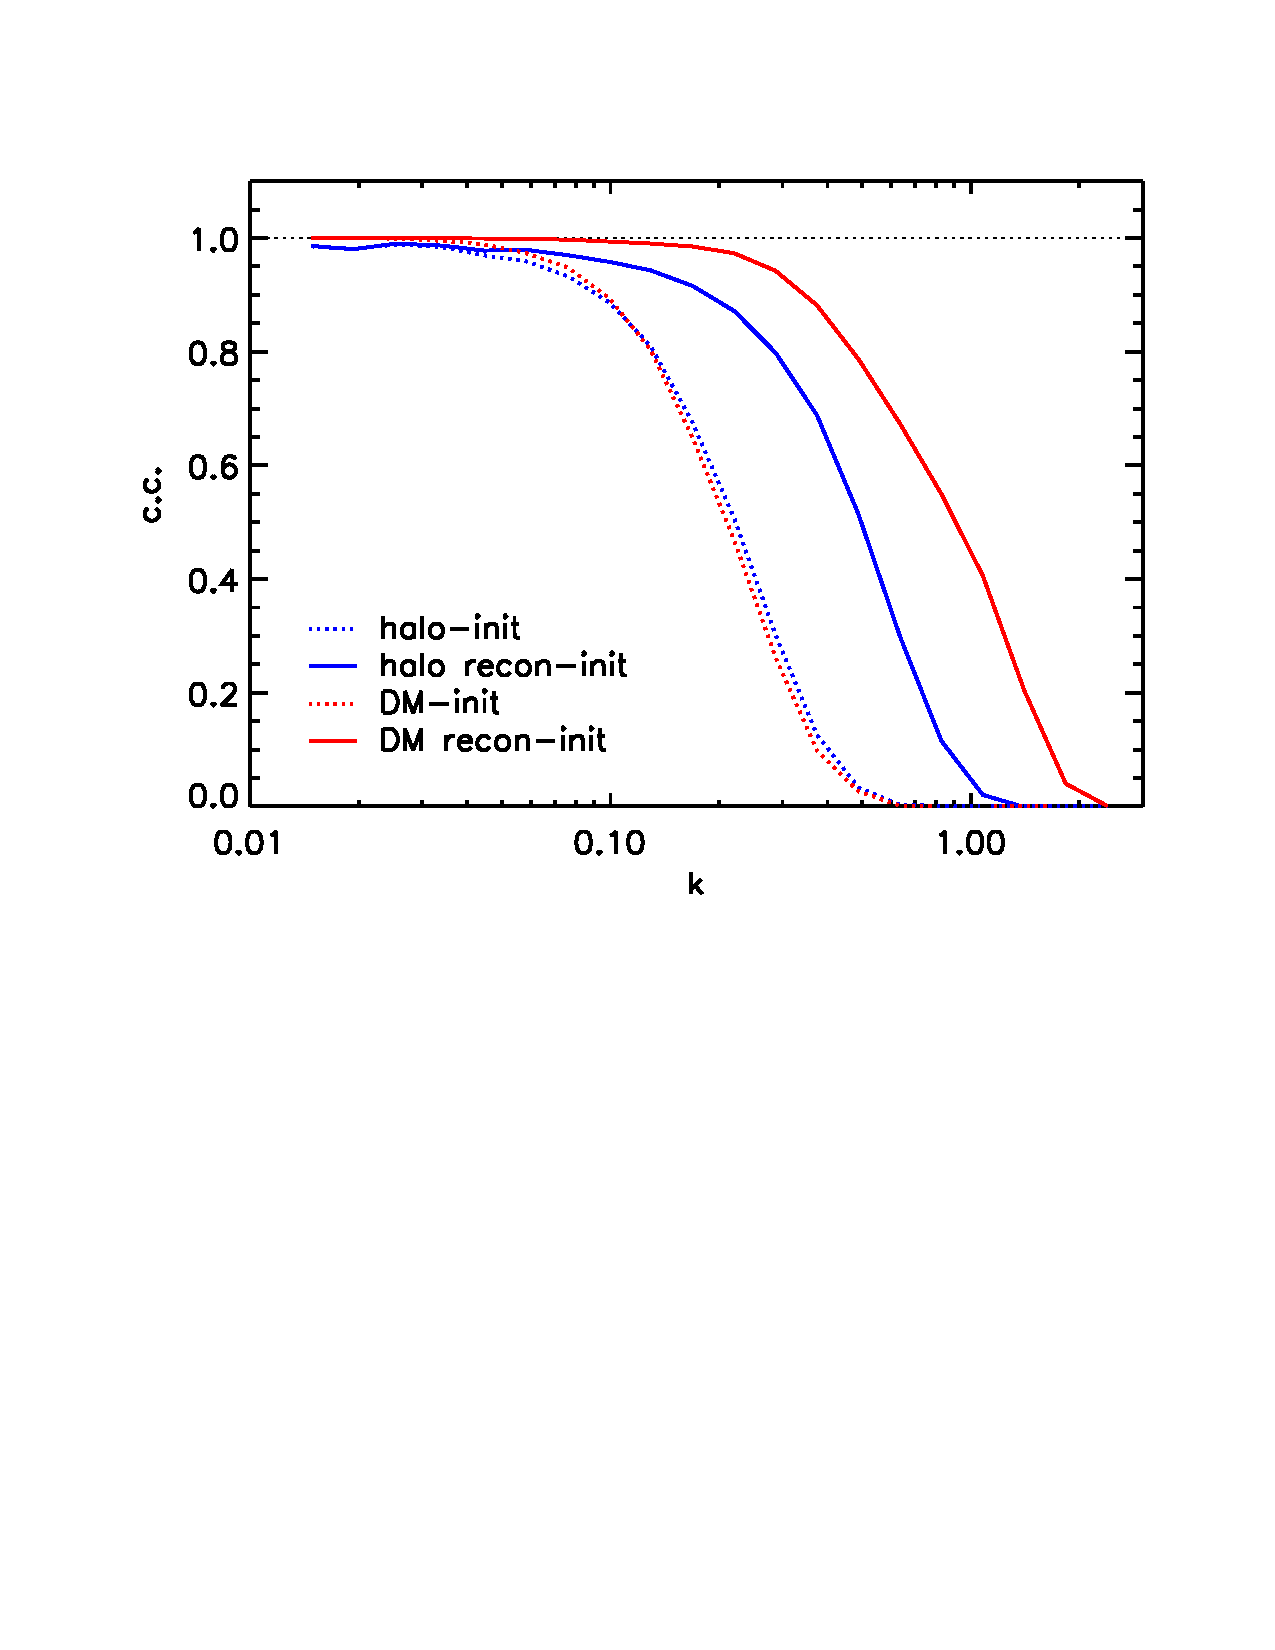
\includegraphics[width=5.0in]{Figures/halocc.pdf}
}

\frame{
\vspace{-0.5in}
    \frametitle{ cosmological applications}
    \begin{itemize}
        \item map initial (linear) tidal-inertia field
        \item BAO, standard ruler (Alcock-Paczynski effect)
        \item modified gravity, neutrino mass, parity violation
     \end{itemize}
  }

  \frame{
    \frametitle{Movie}
    {\tt http://cita.utoronto.ca/\~\,haoran/thnu/movie.html}
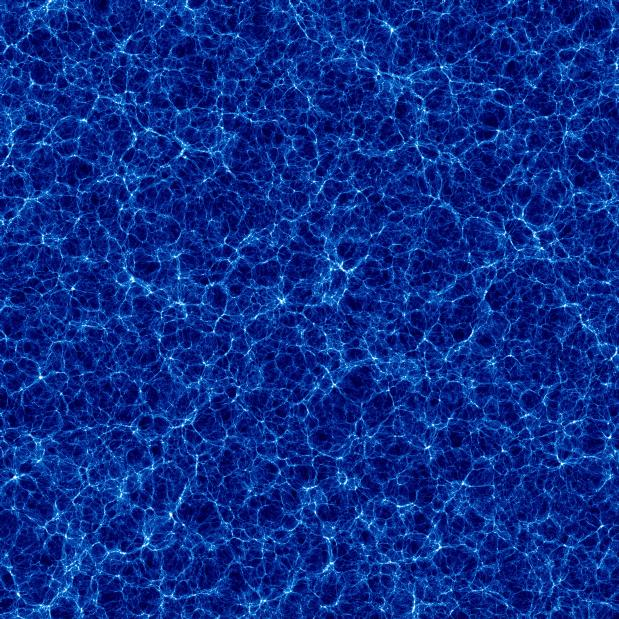
\includegraphics[width=4.2in]{Figures/thnucdmlowres.jpg}
}


\frame{
\vspace{-0.5in}
    \frametitle{Conclusions}
    \begin{itemize}
      \item galaxy spins: new probe of initial conditions
      \item new results on {\it sign} of spin vector: beyond tidal field
      \item predictable from observable displacement field using
        non-linear reconstruction
      \item computationally straightforward, mass coordinate
            similar to Lagrangian
          \item already observable, scalable to much larger surveys
          \item parity odd field, less likely to be contaminated
            (e.g. lensing)
          \item enables measurement of 2 cosmic scalar fields:
            potential beat cosmic variance limits, etc
     \end{itemize}
  }


\end{document}
